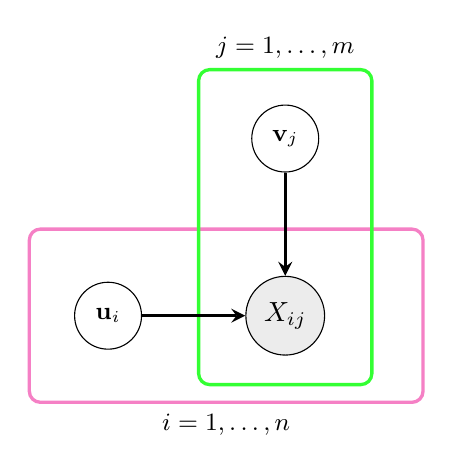
\begin{tikzpicture}[
    scale=1.5,
    node distance=1.5cm,
    >=stealth,
    observed/.style={circle, draw, fill=gray!15, minimum size=1.0cm, font=\normalsize},
    param/.style={circle, draw, fill=white, minimum size=0.85cm, font=\small},
    plate/.style={draw, rectangle, rounded corners, inner sep=8pt, very thick}
]

% Plates first (bottom layer)
% Horizontal plate for i (samples) - longer/wider, magenta
\node[plate, draw=magenta!50, minimum width=5cm, minimum height=2.2cm] (plate_i) at (-0.5, 0) {};
\node[anchor=north, font=\small] at (plate_i.south) {$i = 1, \ldots, n$};

% Vertical plate for j (genes) - narrower/taller, green
\node[plate, draw=green!80, minimum width=2.2cm, minimum height=4cm] (plate_j) at (0, 0.75) {};
\node[anchor=south, font=\small] at (plate_j.north) {$j = 1, \ldots, m$};

% Nodes on top - u and x horizontally aligned, x and v vertically aligned
\node[param] (u) at (-1.5, 0) {$\mathbf{u}_i$};
\node[observed] (x) at (0, 0) {$X_{ij}$};
\node[param] (v) at (0, 1.5) {$\mathbf{v}_j$};

% Arrows (drawn after nodes so they connect properly)
\draw[->, very thick] (u) -- (x);
\draw[->, very thick] (v) -- (x);

\end{tikzpicture}
